\documentclass[compress, red]{beamer}		% \documentclass[compress, red]{beamer}
%\documentclass[compress, red, handout]{beamer}	

\mode<presentation>
\usetheme{Warsaw}							% Beamer theme
\usecolortheme{lily}							% Beamer color theme
\useoutertheme[subsection=false]{smoothbars}		% Beamer outer theme.
										% subsection: add an additional bar for section navigation
\useinnertheme{rectangles}					% Beamer inner theme
\setbeamercovered{transparent}				%Beamer uses transparent overlays
%\setbeamertemplate{footline}[page number]		% Add slide number

\setbeamertemplate{itemize item}[ball]
\setbeamertemplate{itemize subitem}[triangle]
\setbeamertemplate{itemize subsubitem}[circle]

\usepackage[english,frenchb]{babel}
\usepackage[utf8]{inputenc}	% accents under any OS but in TeXShop, requieres preferences/encoding to be set on UTF-8

\usepackage{amsmath}		% for math fonts
\usepackage{graphicx}		% to include figures
\usepackage{subfigure}		% to have figures in figures
\usepackage{multimedia}		% to include movies

\usepackage{hyperref}
\hypersetup{ 
     backref=true,    %permet d'ajouter des liens dans... 
     pagebackref=true,%...les bibliographies 
     hyperindex=true, %ajoute des liens dans les index. 
     colorlinks=false, %colorise les liens 
     breaklinks=true, %permet le retour à la ligne dans les liens trop longs 
     urlcolor= blue,  %couleur des hyperliens 
     linkcolor= blue, %couleur des liens internes 
     bookmarks=true,  %créé des signets pour Acrobat 
     bookmarksopen=true,            %si les signets Acrobat sont créés, les afficher complètement. 
} 

%\usepackage{pstricks}		% to draw
\usepackage{pst-node}

\usepackage{pdftricks}
\begin{psinputs}
   \usepackage{pstricks}
   \usepackage{pst-node}
\end{psinputs}

\usepackage[absolute,overlay]{textpos}

%--------------------------Title Page--------------------------
\title{MetroloJ: an ImageJ plugin to help monitor microscopes' health.}
\author{\href{mailto:fabrice.cordelieres@curie.u-psud.fr}{Cédric Matthews and Fabrice P. Cordelières}}
\date{\textit{3$^{rd}$ ImageJ User and Developer Meeting\\October, the 29th 2010}}

%-------------------Start of the document-------------------
\begin{document}
\frame{					% the title page
	\titlepage
	\vspace{0.2cm}
{\tiny CM: CNRS-IBDML-UMR 6216, Service Imagerie, Marseille, France\\
FPC: Institut Curie/CNRS UMR 3348, PICT-IBiSA@Orsay, Orsay, France\\
CM \& FPC: Mission Ressources et Compétences Technologiques du CNRS, Meudon, France}

	%\begin{center}
		%
\includegraphics[height=2cm]{img/logo-centenaire-bleu-word.jpg}
	%\end{center}
}

%\AtBeginSection{\frame[shrink=35]{\frametitle{Plan}\tableofcontents[currentsection]}}. 

%------------------------The MetroloJ plugins' package----------------------
\setbeamercovered{invisible} 
\section{MetroloJ}
\subsection{The MetroloJ plugins' package}
\frame[shrink=15]{
	\frametitle{The MetroloJ plugins' package}
	\begin{itemize}
		\item<1-> A package of 5 plugins to quantify 4 vital signs of a microscope:
		\begin{itemize}
			\item<2-> Field illumination homogeneity.
			\item<3-> Variability in detection.
			\item<4-> 3D resolutions (including 2 ways to measure axial resolution).
			\item<5-> Images' registration/co-alignement.
		\end{itemize}
		\item<6-> All plugins are based on an unified interface.
		\begin{center}
			\uncover<6->{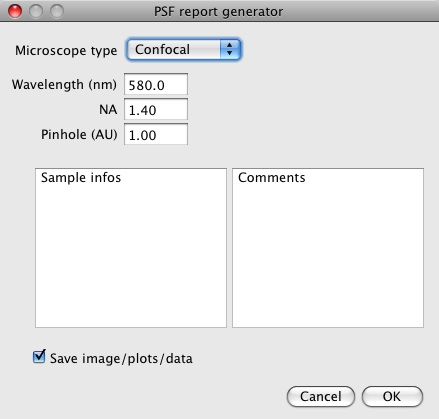
\includegraphics[width=0.4\columnwidth]{./img/gpr-interf}}
		\end{center}
		\item<7-> All plugins provide a unified output in the form of spreadsheets and a pdf file (requires the iText library).
	\end{itemize}
}

%------------------------Field illumination----------------------
\section{Field illumination}
\subsection{Topic 1: Field illumination}
\frame[shrink=15]{
	\frametitle{Topic 1: Field illumination}
	\begin{columns}
		\begin{column}{0.35\textwidth}
			\uncover<3->{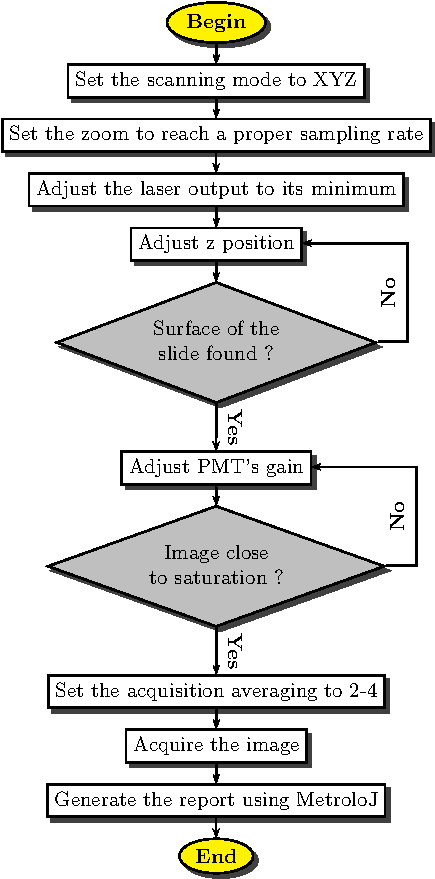
\includegraphics[width=\columnwidth]{MetroloJ-updated-fig2}}
		\end{column}
		\begin{column}{0.65\textwidth}
			\begin{itemize}
				\item<1-> \textbf{Aim:} Check for illumination mis-alignement and/or inhomogeneity.
				\item<2-> \textbf{Sample to be used:} Uniformly fluorescent sample (fluorescent plastic slides, densely packed fluorescent beads...).
				\item<3-> \textbf{Acquisition of a standardized image}.
				\item<4-> \textbf{Informations to be retrieved:}
				\begin{itemize}
					\item<5-> Intensity profiles along the horizontal/vertical axis, diagonals.
					\item<6-> Location of the maximum of intensity and the center of mass.
				\end{itemize}
				\item<7-> \textbf{Preventive/Pro-active actions:} Check the optical path, re-align the light source, ..., call after-sale service.
			\end{itemize}
		\end{column}
	\end{columns}
}

\subsection{Field illumination: what's on the report ?}
\frame[shrink=15]{
	\frametitle{Field illumination: what's on the report ?}
	\begin{figure}
		\begin{center}
			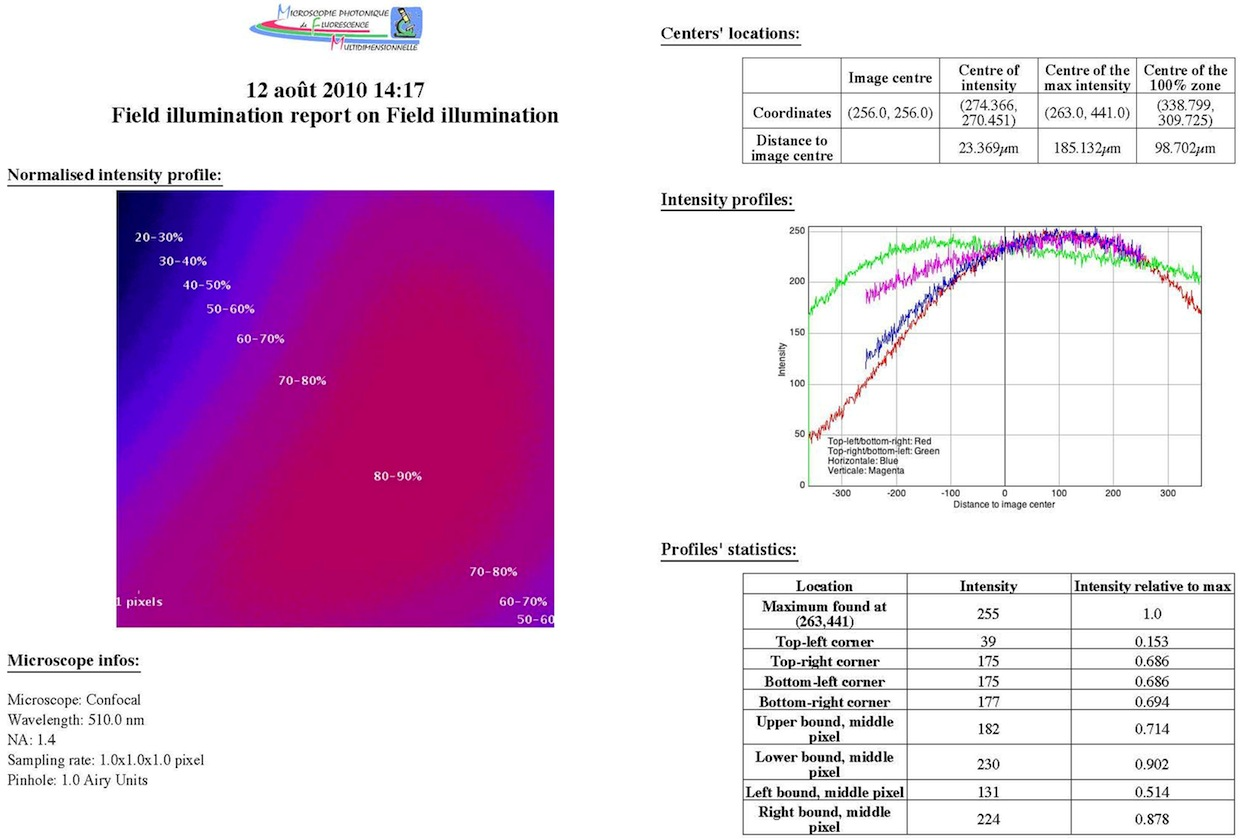
\includegraphics[width=\linewidth]{./img/gfir-report}
		\end{center}
	\end{figure}}

%------------------------Detectors' sensitivity----------------------
\section{Variability in detection}
\subsection{Topic 2: Variability in detection}
\frame[shrink=15]{
	\frametitle{Topic 2: Variability in detection}
	\begin{columns}
		\begin{column}{0.35\textwidth}
			\uncover<3->{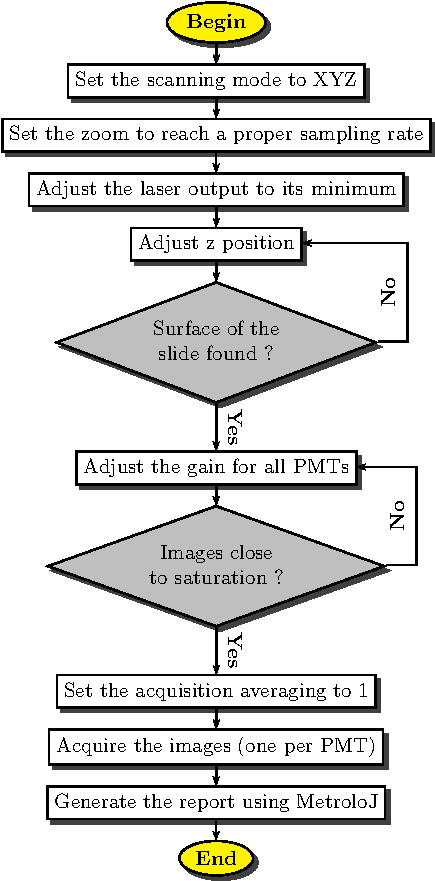
\includegraphics[width=\columnwidth]{MetroloJ-updated-fig1}}
		\end{column}
		\begin{column}{0.65\textwidth}
			\begin{itemize}
				\item<1-> \textbf{Aim:} Using a statistical indicator, the coefficient of variation, (CV) to measure the variability of signal detection.
				\item<2-> \textbf{Sample to be used:} Uniformly fluorescent sample (fluorescent plastic slides, large fluorescent beads...).
				\item<3-> \textbf{Acquisition of a standardized image}.
				\item<4-> \textbf{Informations to be retrieved:} Within a region of interest, mean intensity ($\mu$) and standard deviation . 
				\begin{itemize}
					\item<5-> Average intensity ($\mu$).
					\item<6-> Standard deviation ($\sigma$).
					\item<7-> CV=$\sigma$/$\mu$.
				\end{itemize}
				\item<8-> \textbf{Preventive/Pro-active actions:} Check the optical path, ..., call after-sale service.
			\end{itemize}
		\end{column}
	\end{columns}
}


\subsection{Variability in detection: what's on the report ?}
\frame[shrink=15]{
	\frametitle{Variability in detection: what's on the report ?}
	\vspace{1.25cm}
	\begin{figure}
		\begin{center}
			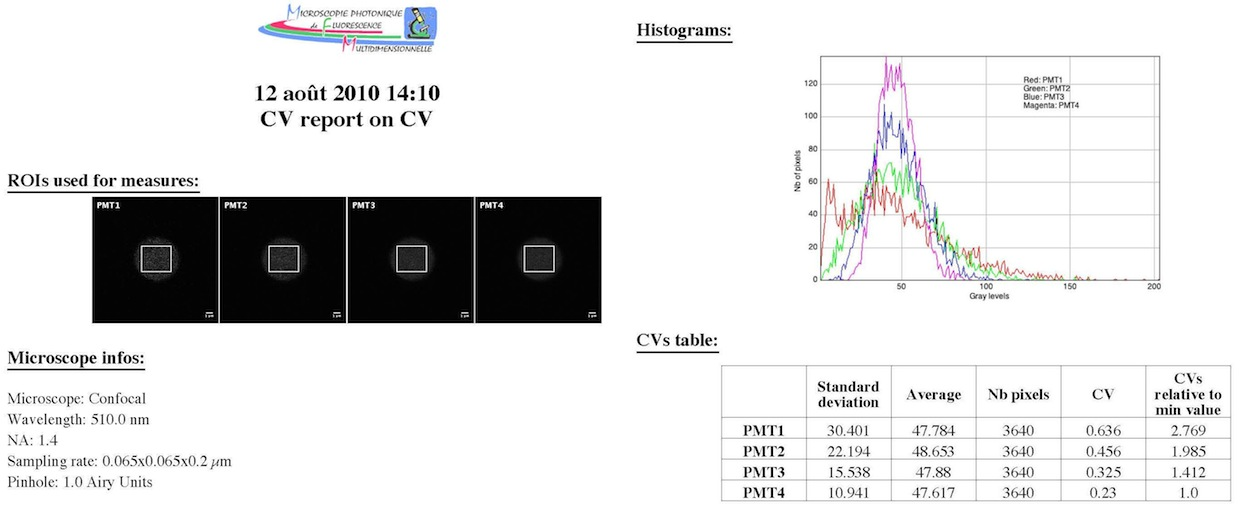
\includegraphics[width=\linewidth]{./img/gcvr-report}
		\end{center}
	\end{figure}}

%------------------------Resolution----------------------
\section{Resolution}
\subsection{Topic 3: Resolution, PSF based measurements}
\frame[shrink=15]{
	\frametitle{Resolution: PSF based measurements}
	\begin{columns}
		\begin{column}{0.35\textwidth}
			\uncover<3->{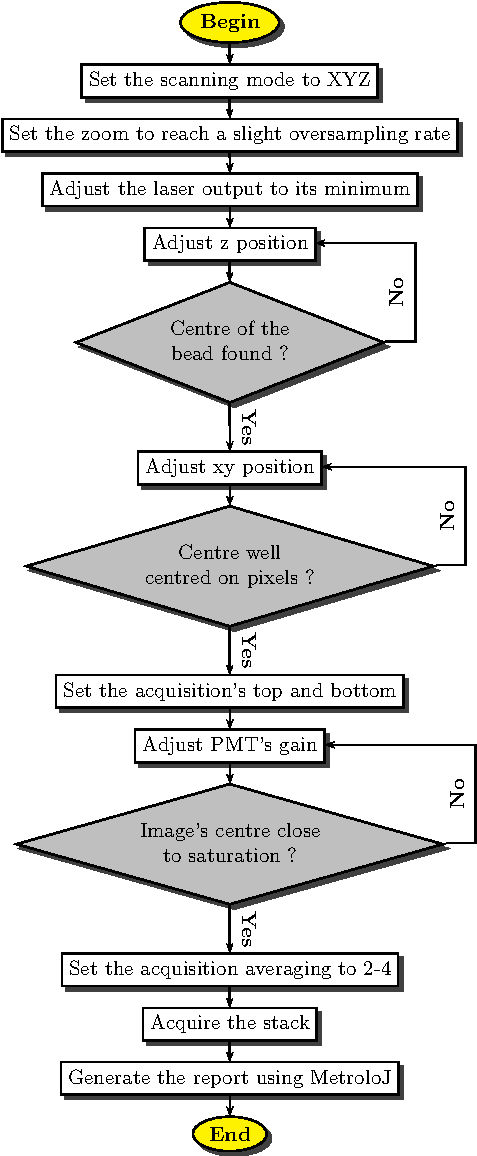
\includegraphics[width=0.8\columnwidth]{MetroloJ-updated-fig3}}
		\end{column}
		\begin{column}{0.65\textwidth}
			\begin{itemize}
				\item<1-> \textbf{Aim:} On the instrumental transfer function, mesure the X, Y and Z resolutions.
				\item<2-> \textbf{Sample to be used:} Well dispersed, uniformly fluorescent labelled, infra-resolution beads.
				\item<3-> \textbf{Acquisition of a standardized image}.
				\item<4-> \textbf{Informations to be retrieved:} Based on intensity profiles passing through the bead's center, fitted on a Gaussian function, determine the FWHM (estimate of the resolution).
				\item<5-> \textbf{Preventive/Pro-active actions:} Check the optical path, check for index mismatches (ex: RI of the immersion oil, mounting medium...), ..., call after-sale service.
			\end{itemize}
		\end{column}
	\end{columns}
}

\subsection{PSF based measurements: what's on the report ?}
\frame[shrink=15]{
	\frametitle{PSF based measurements: what's on the report ?}
	\begin{figure}
		\begin{center}
			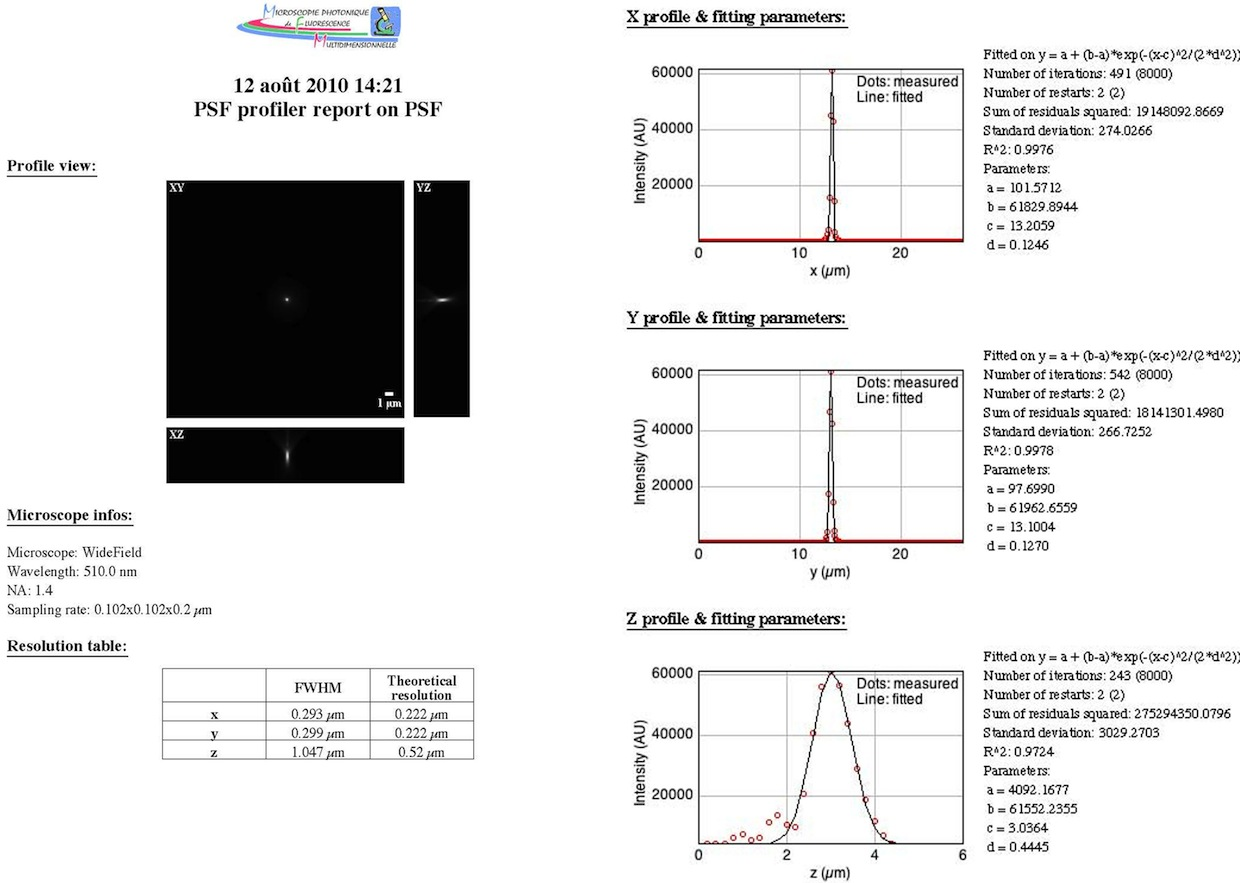
\includegraphics[width=\linewidth]{./img/gpr-report}
		\end{center}
	\end{figure}
}

\subsection{Topic 3: Resolution, mirror slide based measurement}
\frame[shrink=15]{
	\frametitle{Resolution: Mirror slide based measurement}
	\begin{columns}
		\begin{column}{0.35\textwidth}
			\uncover<3->{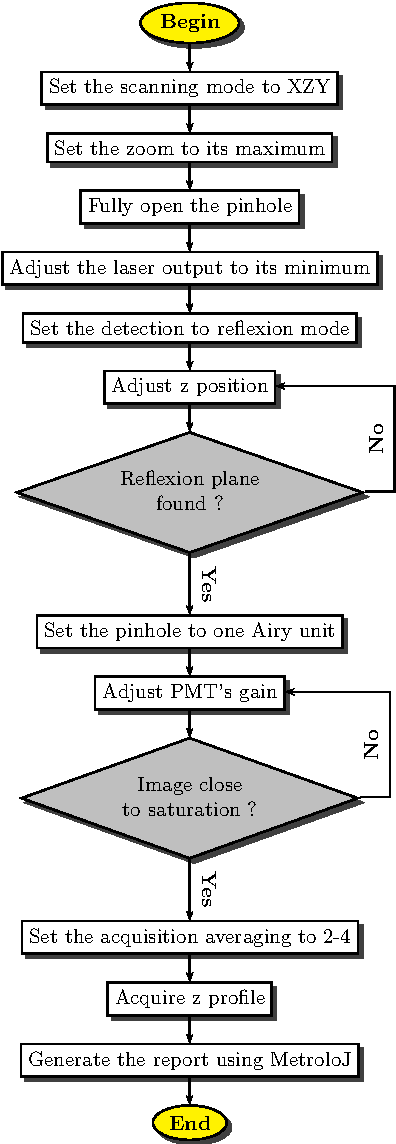
\includegraphics[width=0.7\columnwidth]{MetroloJ-updated-fig4}}
		\end{column}
		\begin{column}{0.65\textwidth}
			\begin{itemize}
				\item<1-> \textbf{Aim:} On a XZ reflexion pattern obtained imaging a mirror, mesure the Z resolution.
				\item<2-> \textbf{Sample to be used:} A plane mirror slide.
				\item<3-> \textbf{Acquisition of a standardized image}.
				\item<4-> \textbf{Informations to be retrieved:} Based on an averaged intensity profiles across the reflexion profile, fitted on a Gaussian function, determine the FWHM (estimate of the resolution).
				\item<5-> \textbf{Preventive/Pro-active actions:} Check the optical path, check for index mismatches (ex: RI of the immersion oil, mounting medium...), ..., call after-sale service.
			\end{itemize}
		\end{column}
	\end{columns}
}

\subsection{Mirror slide based measurement: what's on the report ?}
\frame[shrink=15]{
	\frametitle{Mirror slide based measurement: what's on the report ?}
	\begin{figure}
		\begin{center}
			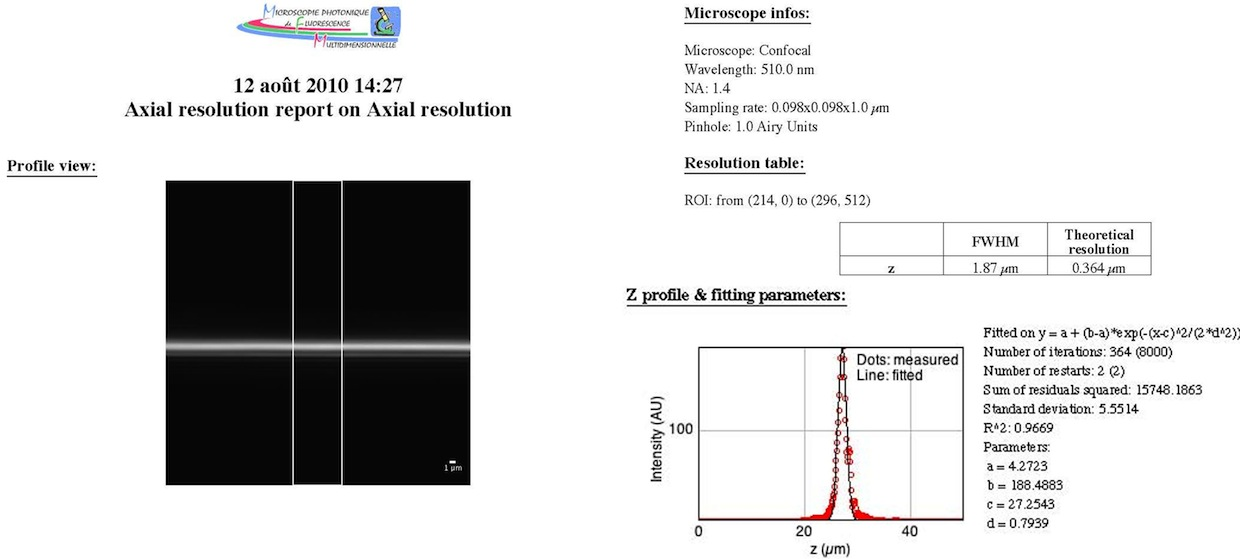
\includegraphics[width=\linewidth]{./img/garr-report}
		\end{center}
	\end{figure}
}

%------------------------Co-alignement----------------------
\section{Co-alignement}
\subsection{Topic 4: Co-alignement}
\frame[shrink=15]{
	\frametitle{Topic 4: Co-alignement}
	\begin{columns}
		\begin{column}{0.35\textwidth}
			\uncover<3->{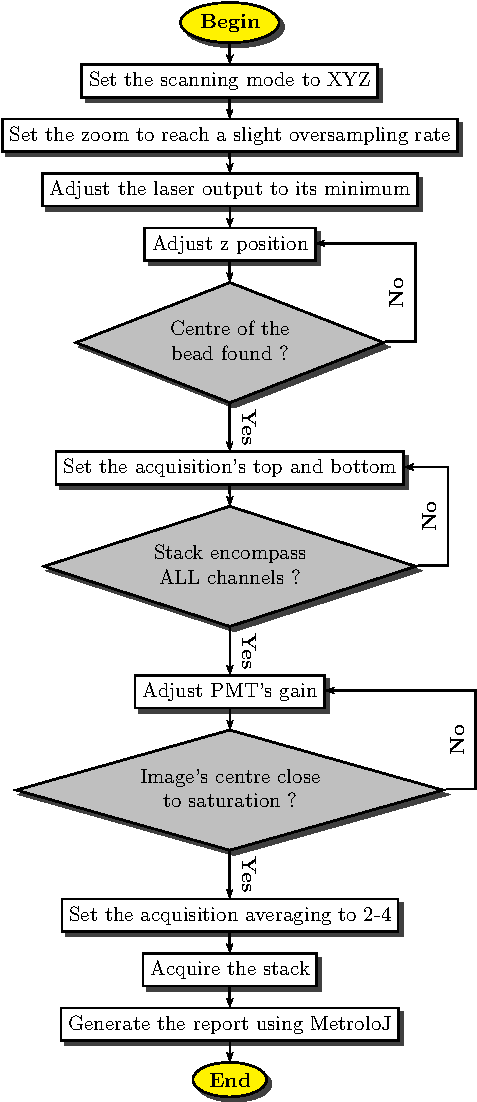
\includegraphics[width=0.85\columnwidth]{MetroloJ-updated-fig5}}
		\end{column}
		\begin{column}{0.65\textwidth}
			\begin{itemize}
				\item<1-> \textbf{Aim:} On the image of a multi-labelled objet, measure the distances between images of the different channels.
				\item<2-> \textbf{Sample to be used:} Well dispersed, uniformly fluorescent labelled, large beads.
				\item<3-> \textbf{Acquisition of a standardized image}.
				\item<4-> \textbf{Informations to be retrieved:} For each channel:
				\begin{itemize}
					\item<5->Position of the bead's center geometrical center.
					\item<6-> For each pair of channels, uncalibrated (pixels) and calibrated($\mu$m) center to center distances
				\end{itemize}
				\item<7-> \textbf{Preventive/Pro-active actions:} Check the optical path, re-align the light source, check for index mismatches (ex: RI of the immersion oil, mounting medium...), ..., call after-sale service.
			\end{itemize}
		\end{column}
	\end{columns}
}


\subsection{Co-alignement: what's on the report ?}
\frame[shrink=15]{
	\frametitle{Co-alignement: what's on the report ?}
	\begin{figure}
		\begin{center}
			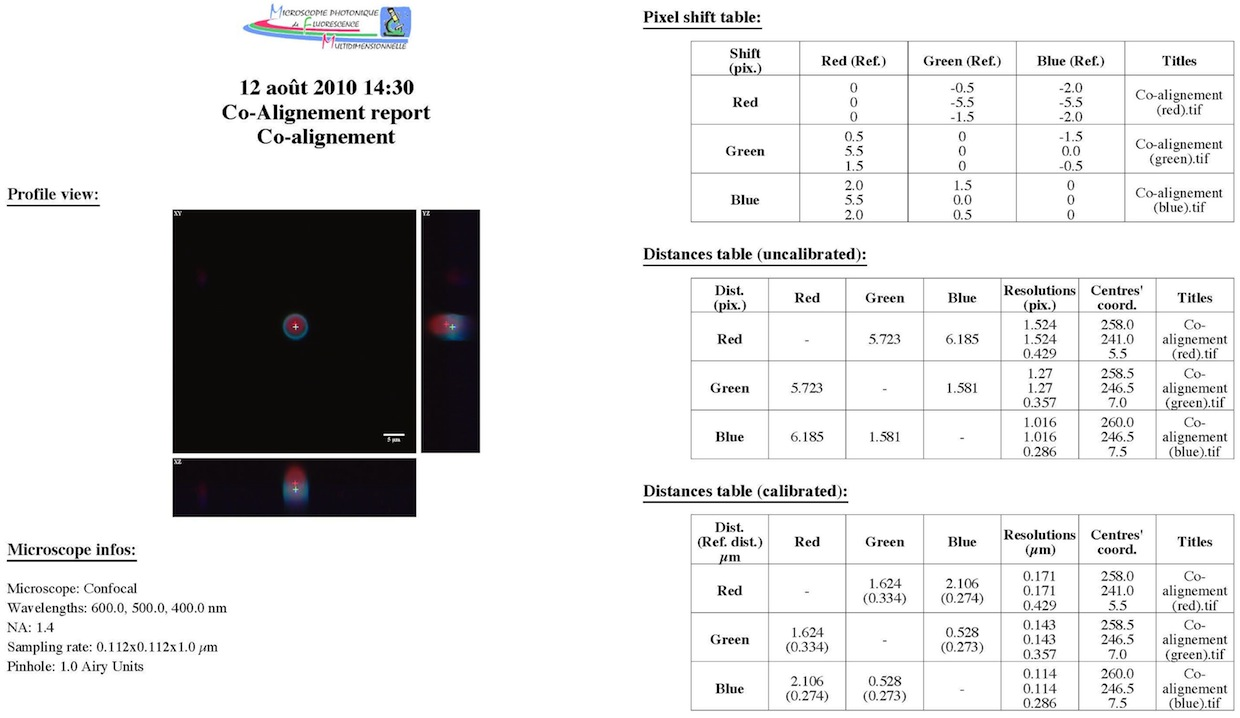
\includegraphics[width=\linewidth]{./img/gcoar-report}
		\end{center}
	\end{figure}}

%------------------------Future work----------------------
\section{Conclusions, ongoing/future works}
\subsection{Why and when should the MetroloJ package be used ?}
\frame[shrink=15]{
	\frametitle{Why and when should the MetroloJ package be used ?}
	\textbf{\textit{The MetroloJ package is a collection of plugins aimed at extracting quantitative data out of images taken on standardized samples, using standardized procedures.}}
	\vspace{0.5cm}
	\begin{itemize}
		\item<2-> \textbf{\textit{Before purchasing a new system:}}
		\begin{itemize}
			\item<3-> Define expected performances.
			\item<4-> Measure/test for the actual performances of the candidates.
			\item<5-> Compare systems in a standardized fashion.
			\item<6-> Make a choice based on quantitative, non subjective criterions.
		\end{itemize}
		\vspace{0.25cm}
		\item<7-> \textbf{\textit{After purchase: system monitoring:}}
		\begin{itemize}
			\item<8-> \textit{Upon equipment reception:}
			\begin{itemize}
				\item<9-> Check for fulfillment of the performances' expectations.
			\end{itemize}
			\item<10-> \textit{All along the equipment's lifetime:}
			\begin{itemize}
				\item<11-> Check for stability.
				\item<12-> Prevent downtimes.
				\item<13-> Take preventive/pro-active measures.
			\end{itemize}
		\end{itemize}
	\end{itemize}
}

%------------------------Future work----------------------
\subsection{Ongoing/future works}
\frame{
	\frametitle{Ongoing/future works}
	\begin{itemize}
		\item<1-> \textbf{\textit{New tests:}}
		\begin{itemize}
			\item<2-> Check for microscope's stage drift (one position, over time).
			\item<3-> Check for microscope's stage proper re-positionning (several positions, revisited n times).
			\item<4-> Measure of detectors response curves.
		\end{itemize}
		\vspace{0.25cm}
		\item<5-> \textbf{\textit{Data archiving, systems' benchmarking:}}
		\begin{itemize}
			\item<6-> Option: send measures to a database
			\item<7-> From the database, get an estimate of the ``normal'' situation to which each single measure might be compared to.
		\end{itemize}
	\end{itemize}
}

\subsection{Acknowledgments}
\frame[shrink=20]{
	\frametitle{Acknowledgments}
	\textbf{\textit{Thanks to all the members of the `groupe de travail Métrologie du RT-MFM'' and/or of the MetroloJ package's beta-testers... (and all apologies for the potentially forgotten ones).}}
	\vspace{0.5cm}
	\begin{columns}
		\begin{column}{0.5\textwidth}
			\begin{itemize}
				\item Pierre Bourdoncle
				\item Anne Cantereau
				\item Julien Cau
				\item Christophe Chamot
				\item Julien Cianfichi
				\item Aurélien Dauphin
				\item Olivier Duc
				\item Sylvain De Rossi
				\item Stéphanie Dutertre
				\item Aude Jobart-Malfait
				\item Christophe Klein
				\item Marc Lartaud
				\item Patricia Le Baccon
			\end{itemize}
		\end{column}
		\begin{column}{0.5\textwidth}
			\begin{itemize}
				\item Aurélie Le Ru
				\item Meriem Garfa-Traoré
				\item Camille Lebugle
				\item Sandrine Leveque-Fort
				\item Christophe Machu
				\item Laure Malicieux
				\item Christel Poujol
				\item Richard Schwartzmann
				\item Damien Schapman
				\item Marie-Noëlle Soler
				\item Nicolas Tissot
				\item Yves Usson
				\item Fran\c cois Waharte
			\end{itemize}
		\end{column}
	\end{columns}
}



\end{document}